\documentclass[a4paper,11pt]{ltjsarticle}

\usepackage[margin=25mm]{geometry}
\usepackage{graphicx}
\usepackage{hyperref}
\usepackage{enumitem}
\usepackage{parskip}

\hypersetup{
  colorlinks=true,
  linkcolor=blue,
  urlcolor=blue,
  pdftitle={オーディオシステムにおけるケーブル起因劣化を扱う研究指向シミュレーション枠組み},
  pdfauthor={moe-charm}
}

\setlist{nosep}

\title{オーディオシステムにおけるケーブル起因劣化を扱う\\研究指向シミュレーション枠組み}
\author{moe-charm}
\date{\today}

\begin{document}

\maketitle

\begin{abstract}
本稿では、ケーブル物理、インターフェース負荷、アンプ挙動、時間領域
DSP近似、そして聴感寄りの指標を、一つの解析・試聴パイプラインへ統合
した研究指向のオーディオシステム・シミュレータを示す。目的は、報告
されるすべてのケーブル差を説明し切ったと主張することではなく、ケー
ブル起因の劣化がどのような条件でシステム全体に現れうるかを、構造化
かつ検証可能な形で扱うことである。

本フレームワークは、RLGCに基づくケーブルモデルに加え、ライン段の相互
作用、小信号アンプのストレス、非線形アンプ挙動、誘電吸収、熱変調、
共通リターン汚染、複雑スピーカー負荷を組み合わせる。これにより、
周波数特性、群遅延、インパルス応答、ステップ応答、TailRatio、
StageError、ダンピングファクター、駆動力ロス、クロストーク推定、
シールド侵入推定などを導出できる。

現時点でも本シミュレータは、長尺または劣化したRCAや、極端に長い
スピーカーケーブルのような厳しい条件下で、単なる音量差を超える劣化を
再現できる。一方で、筆者が経験した「こもり」「高域の艶や伸び」
「音場の変化」「濃い音」といった、より繊細な聴感差は、まだ十分に納得
できる条件で再現できていない。したがって本研究は、完成した証明では
なく、統合シミュレーション基盤および仮説生成ツールとして位置づけられる。
\end{abstract}

\textbf{キーワード:} オーディオケーブル，インターフェース負荷，アンプ相互作用，
RLGC，群遅延，インパルス応答，研究用シミュレータ

\section{はじめに}

ケーブルによる音の違いに関する議論は、しばしば二つの極端な立場に分か
れる。すなわち、すべてを物理的に無意味とみなす立場と、すべてを主観的
事実として受け入れる立場である。本研究はその中間に立ち、ケーブル単体
ではなく、システム全体の相互作用として理解できる現象がどこまであるか
を調べる。

とくに、数m程度のケーブル長そのものが可聴な伝搬遅延を直接生むとは考え
にくい。しかし、ケーブル容量、リターン電流、セトリング、アンプのルー
プストレス、ダンピング、負荷相互作用などを通じて、接続された機器の動
作条件を変えることはありうる。その結果として、こもり、駆動力低下、
過渡応答の軟化、音像の甘さといった聴感上の変化が生じる可能性がある。

本稿の貢献は、すべての聴感差を最終的に説明したことではない。ケーブル、
機器相互作用、DSP近似、聴感指標を一つの枠組みに収め、解析と試聴を同じ
チェーン上で扱えるようにした点にある。

\section{主張の範囲}

本研究が現時点で主張するのは、以下の範囲に限られる。

\begin{itemize}
  \item 極端に悪いケーブル条件では、音質劣化を数値的にも聴感上も再現しやすい
  \item ケーブル差の一部は、導体抵抗そのものよりも機器との相互作用で説明しやすい
\end{itemize}

逆に、以下はまだ主張しない。

\begin{itemize}
  \item すべてのケーブル聴感報告が正しいこと
  \item すべての聴感差を現モデルが説明できること
  \item 現在のシミュレータが実測的に完成していること
\end{itemize}

この境界を明確にすることが、本稿の前提である。

\section{フレームワーク概要}

現在の信号チェーンは以下の通りである。

\begin{enumerate}
  \item ライン段ケーブル伝達
  \item ライン段の誘電吸収
  \item 共通リターン汚染
  \item シールド侵入ベールと接点劣化汚染
  \item 小信号アンプ応答
  \item 非線形アンプ応答
  \item スピーカーケーブル伝達
  \item スピーカー側の誘電吸収
  \item 熱変調
\end{enumerate}

このチェーンは、グラフ描画用解析と試聴用処理で共有されている。

\begin{figure}[t]
  \centering
  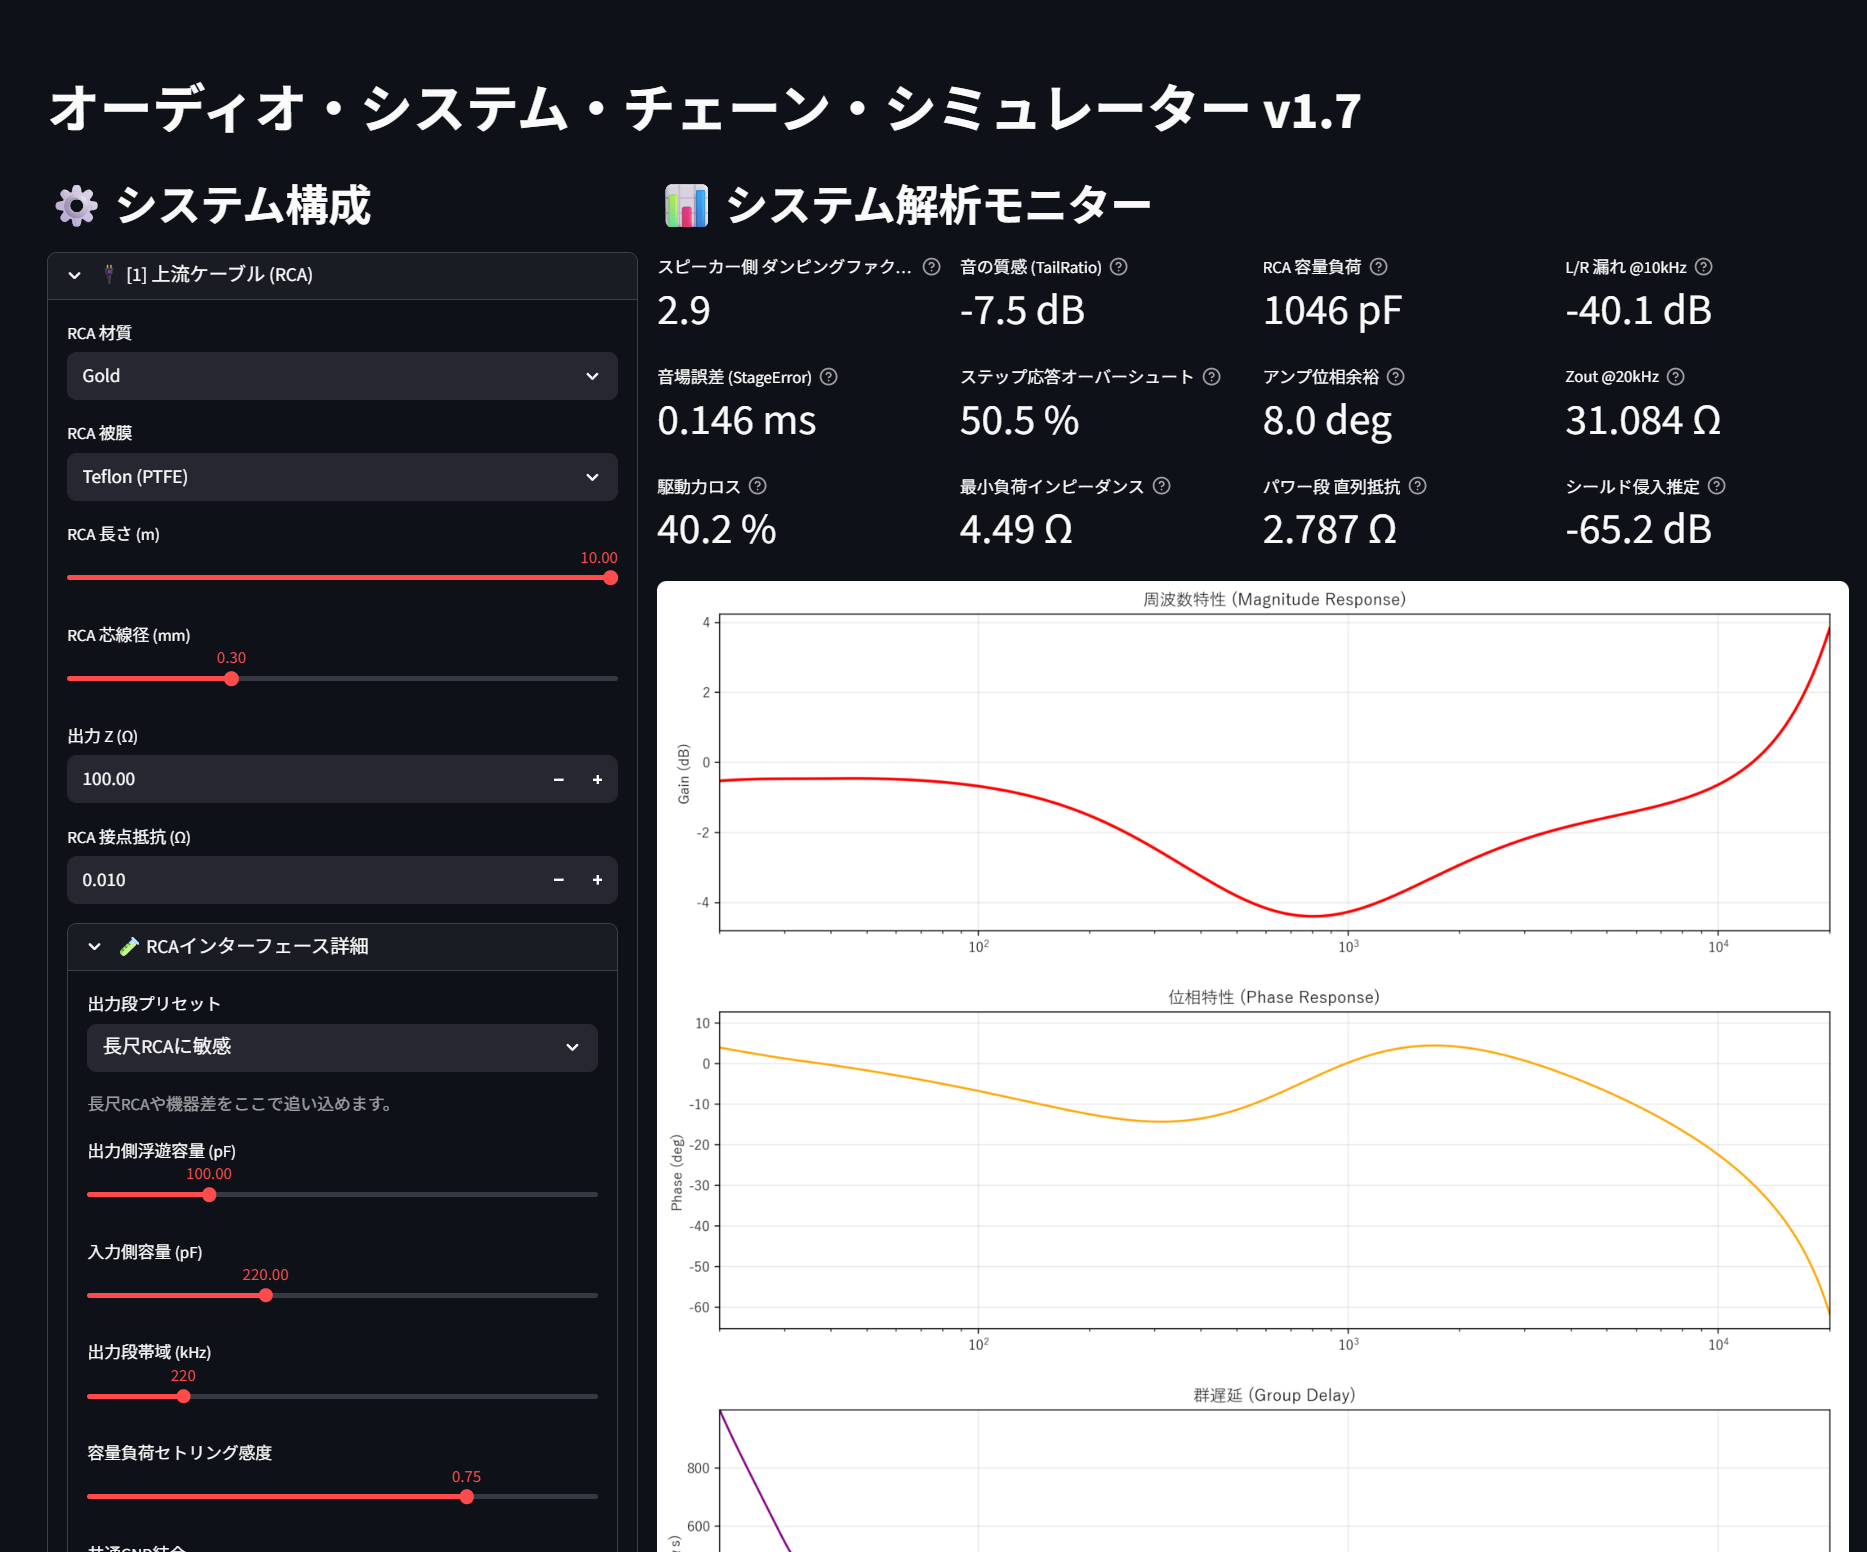
\includegraphics[width=\linewidth]{../../docs/images/app-screenshot.png}
  \caption{現在のStreamlitアプリケーション画面。パラメータ調整、解析、試聴を一体で扱う。}
  \label{fig:app-ui-ja}
\end{figure}

\section{モデル構成}

\subsection{ケーブルモデル}

ケーブルモデルはRLGCを基礎とし、導体材質、構造、被膜、接点抵抗、長さ
で規定される。総容量、総インダクタンス、直流直列抵抗、リターン
インピーダンス、伝達関数を扱う。

\subsection{インターフェースモデル}

ライン段モデルは、出力インピーダンス、入力インピーダンス、浮遊容量、
セトリング、共通リターン結合、シールド品質ストレス、接点劣化推定を
含む。これは、安価または劣化した長尺RCAが、単純な1ポール低域通過以上
の「こもり」を示しうる理由を扱うためのブロックである。

\subsection{アンプモデル}

アンプについては二つの見方を併用する。

\begin{itemize}
  \item 小信号モデルでは、ループストレス、極移動、位相余裕、周波数依存の出力インピーダンスを扱う
  \item 非線形モデルでは、スルーレート制限、電源サグ、高調波付加を扱う
\end{itemize}

これにより、ケーブルや負荷の条件がアンプ挙動へ反映される。

\subsection{スピーカー負荷モデル}

複雑スピーカー負荷モデルは、共振、インダクティブな立ち上がり、
逆起電力風の挙動、クロスオーバー風の分岐を近似する。これにより、
長尺スピーカーケーブルが単に音量を下げるだけでなく、制動不足や
押し出し不足として感じられる理由を追いやすくする。

\subsection{聴感寄り指標}

現在の枠組みでは、以下の指標を扱う。

\begin{itemize}
  \item TailRatio
  \item StageError
  \item ダンピングファクター
  \item 駆動力ロス
  \item クロストーク推定
  \item シールド侵入推定
  \item 位相余裕推定
  \item 20 kHz における出力インピーダンス
  \item インパルス応答およびステップ応答指標
\end{itemize}

これらは知覚の証明そのものではなく、物理変化と聴感語彙をつなぐ橋として
用いる。

\section{現時点の結果}

現実装でも、以下のような傾向はすでに確認できる。

\begin{itemize}
  \item 長尺または劣化したRCAでは、高域減衰、尾部悪化、侵入・接点指標の悪化が生じうる
  \item 極端に長いスピーカーケーブルでは、ダンピングファクター低下や駆動力ロス増大が見える
  \item 複雑負荷モデルを入れると、単純RL負荷よりも「制動が抜ける」変化を再現しやすい
  \item 極端条件では、音質劣化を聴感的にもわかりやすく再現できる
\end{itemize}

一方で、筆者が実際に経験したすべてのケーブル差を、十分説得的な条件で
再現できているわけではない。特に、「こもり」「高域の艶や伸び」
「音場の変化」「濃い音」といった性質は、まだ部分的な説明にとどまる。

\section{今後の検証計画}

今後は、少なくとも以下の検証が必要である。

\begin{enumerate}
  \item RCA長やスピーカーケーブル長を変えたベンチ測定
  \item 容量負荷を変えたときのステップ応答や矩形波応答の比較
  \item 容量・シールド・接点を切り分けるアブレーション実験
  \item 実測インピーダンスの読み込み
  \item 可能であれば統制された試聴実験
\end{enumerate}

\section{限界}

現実装には重要な限界が残っている。

\begin{itemize}
  \item スピーカー負荷はまだ合成モデルであり、実測ベースではない
  \item RF侵入やハムは確率的な実ノイズとしては扱えていない
  \item 接点劣化は断続的故障ではなく、滑らかな近似にとどまる
  \item 実アンプのボード線図はまだ直接取り込めていない
  \item 聴感との対応づけは未完成である
\end{itemize}

これらは単なる但し書きではなく、主張の境界そのものである。

\section{結論}

本研究は、ケーブル起因劣化をオーディオシステム全体の相互作用として扱う
ための統合シミュレーション枠組みを提示した。現時点での結論は限定的だが、
それでも意味は大きい。

まず、極端な条件下では、音質劣化を聴感上でもわかりやすく再現できた。
これは、ケーブルをひどい条件で用いた場合に音が劣化しうるという実務的な
主張を支持する。

しかし、筆者が経験したケーブルによる音のこもり、高域の艶や伸び、音場の
変化、濃い音といった性質は、まだ十分に納得できる条件で再現できていない。
したがって、これらは今後さらに研究すべき課題である。

本研究の価値は二つある。第一に、曖昧な議論を、点検・拡張・実測比較可能
な構造化モデルへ置き換えたこと。第二に、すでに再現できたことと、まだ
説明できていないことを明確に切り分けたことである。第一報としては、
それで十分に意味がある。

\section*{謝辞}

実装および原稿整理の過程では、ChatGPT および Gemini との反復的な技術
議論と開発支援を受けた。これらは研究著者ではなく、開発補助ツールとして
位置づける。

\end{document}

